\section[TargetProcess]{TargetProcess}
Targetprocess é ferramenta para gerenciamento de projeto visual que se concentra na metodologia ágil de desenvolvimento de software com suporte para Scrum, Kanban e SAFe. O software pode ser personalizado atender trabalhos e projetos específicos. 

A equipe fez uso desta ferramenta e, o primeiro passo foi a criação dos quadros para o gerenciamento, como mostra a figura abaixo.

\begin{figure}[!htb]
    \centering
    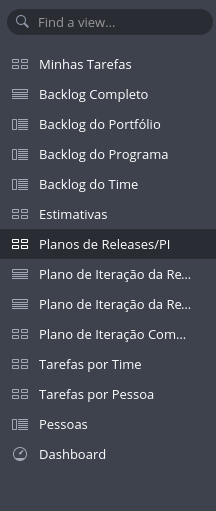
\includegraphics[width=0.2\textwidth]{figuras/quadros.png}
    \caption{Quadros Criados e Utilizados no TargetProcess}
    \label{fig:quadros}
\end{figure}

A partir do TargetProcess, também é possível visualizar o status do projeto no presente momento, com detalhes como: a porcentagem de processos já concluída, features e histórias de usuário realizadas e faltantes, bugs e os criadores/desenvolvedores. Exemplo na próxima imagem.

\begin{figure}[!htb]
    \centering
    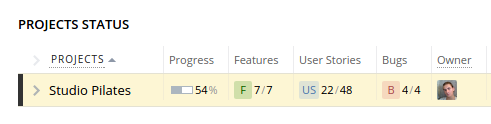
\includegraphics[width=0.7\textwidth]{figuras/status_projeto.png}
    \caption{Status do Projeto}
    \label{fig:status_projeto}
\end{figure}

Além disso, na imagem seguinte, é possível visualizar também o Gráfico Burn Down (também gerado a partir do TargetProcess) que representa diariamente o progresso do trabalho em desenvolvimento. O gráfico da equipe revela que o trabalho ritmo de trabalho foi adequado para atingir a meta da Sprint 1.

\begin{figure}[!htb]
    \centering
    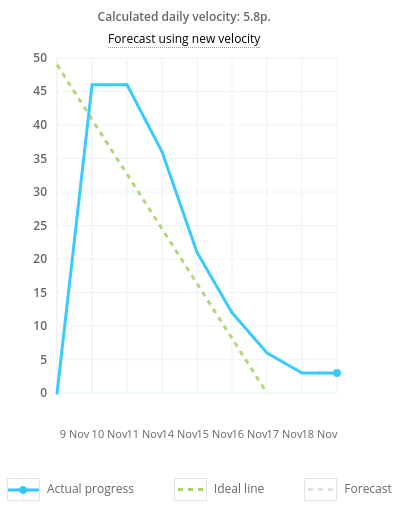
\includegraphics[width=0.5\textwidth]{figuras/burn_down.png}
    \caption{Gráfico Burn Down}
    \label{fig:burn_down}
\end{figure}